\chapter[Okra: Our Solution Proposal]{Okra: Our Solution Proposal}
\label{cp:okra-solution}

{
\parindent0pt

\section{Core Concept and Functionality}
Okra is a mobile-first, web-enabled platform designed as a comprehensive ecosystem to mitigate PHL. The platform serves three primary user groups:

\begin{description}
    \item[Farmers/Producers:] Can create profiles, list their produce (crop type, quantity, harvest date, location), upload images for AI assessment, set indicative prices, and view market demand.
    
    \item[Buyers] Can search for specific produce based on type, quantity, quality (informed by AI score), and location. They can connect with farmers, negotiate, and arrange purchases. Buyers include wholesalers, retailers, processors, and direct consumers.
    
    \item[Logistics Providers] Can register their services (vehicle type – including refrigerated options, capacity, operational routes, pricing). The platform facilitates matching them with farmers/buyers needing transport.
\end{description}

\subsection{Marketplace Networking}
Farmers and producer groups register on the app to list available produce (crop type, quantity, harvest date). Buyers – including wholesalers, processors, and retailers – can search and place orders by region and crop. By centralizing listings, the app ensures farmers find customers quickly, and buyers can discover sources of fresh produce. This reduces unsold inventory and match supply to demand in real time.

\subsection{Logistics Integration}
The app includes a dashboard for logistics providers (truckers, couriers, cold-chain operators). When a sale is made, the system can automatically offer transport jobs to verified drivers. Users can see available vehicles, rates, and track shipments. For example, a farmer in Kano could schedule a refrigerated truck to deliver tomatoes to Lagos. This ensures reliable transport capacity and route planning, cutting delays that lead to spoilage.

\subsection{AI-Powered Insights}
A novel AI feature uses computer vision to analyze produce quality. Farmers or cooperatives upload smartphone images of their harvest batches. The app’s AI model assesses freshness (e.g. spotting bruises, mold, color) and estimates volume or weight from the images. This accomplishes two goals: (1) It provides an objective quality grade for buyers to see, increasing trust. (2) It forecasts how long the produce will remain saleable. The model improves over time as more labeled images are fed back, refining its predictions.

\subsection{Youth-led Agribusiness Empowerment}
The platform encourages youth entrepreneurship. For example, tech-skilled youth can be trained to help digitize farms (taking images, using the app), to become last-mile delivery drivers, or to manage aggregation hubs. The platform could partner with agricultural colleges or startup incubators to recruit graduates. By framing agriculture as a tech-enabled business, the app draws young people into value chains. In effect, it transforms farming from subsistence into a connected, data-driven marketplace, which is more attractive to the next generation.

\begin{block}[note]
    \textit{Because of the time span of the hackathon, development of the Okra web app is not complete. Part of the frontend and most of the backend are still in development. The following sections show the current state of the project, including the mockups and the data strategy.}
    \end{block}


\section{Screens}


\begin{figure}[H]
    \centering
    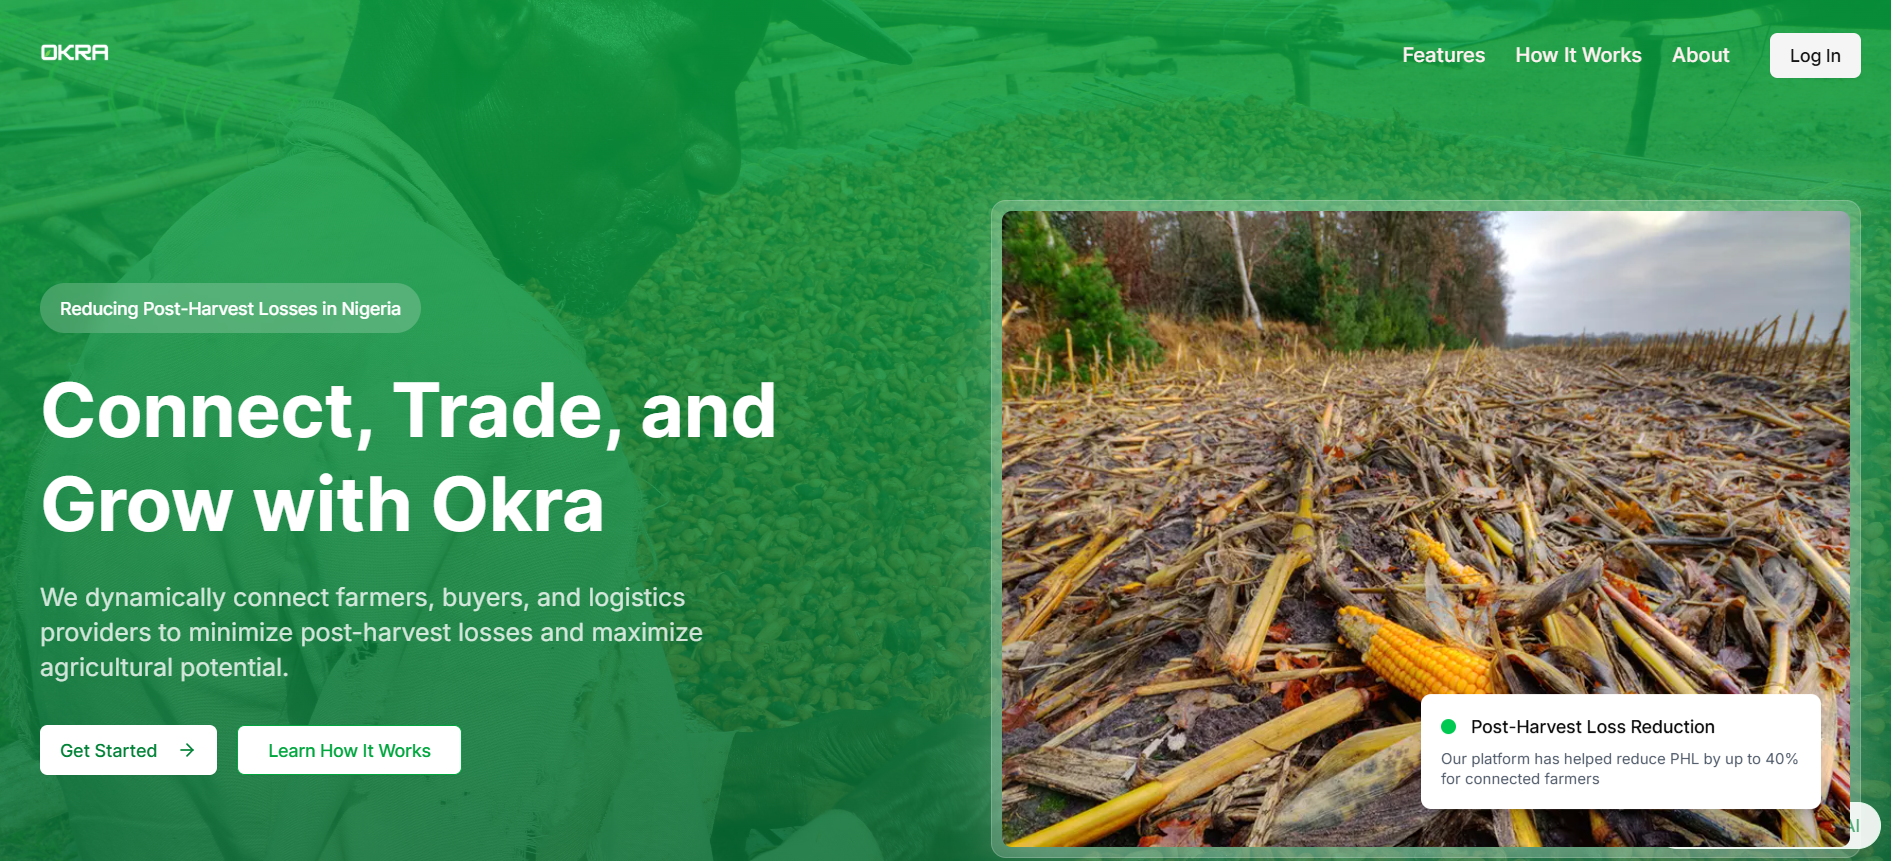
\includegraphics[scale=0.3]{Figures/okra_mockup_landing.png}
    \caption{Screenshot of the landing page}
    \label{fig:figure-05}
\end{figure}


\begin{figure}[H]
    \centering
    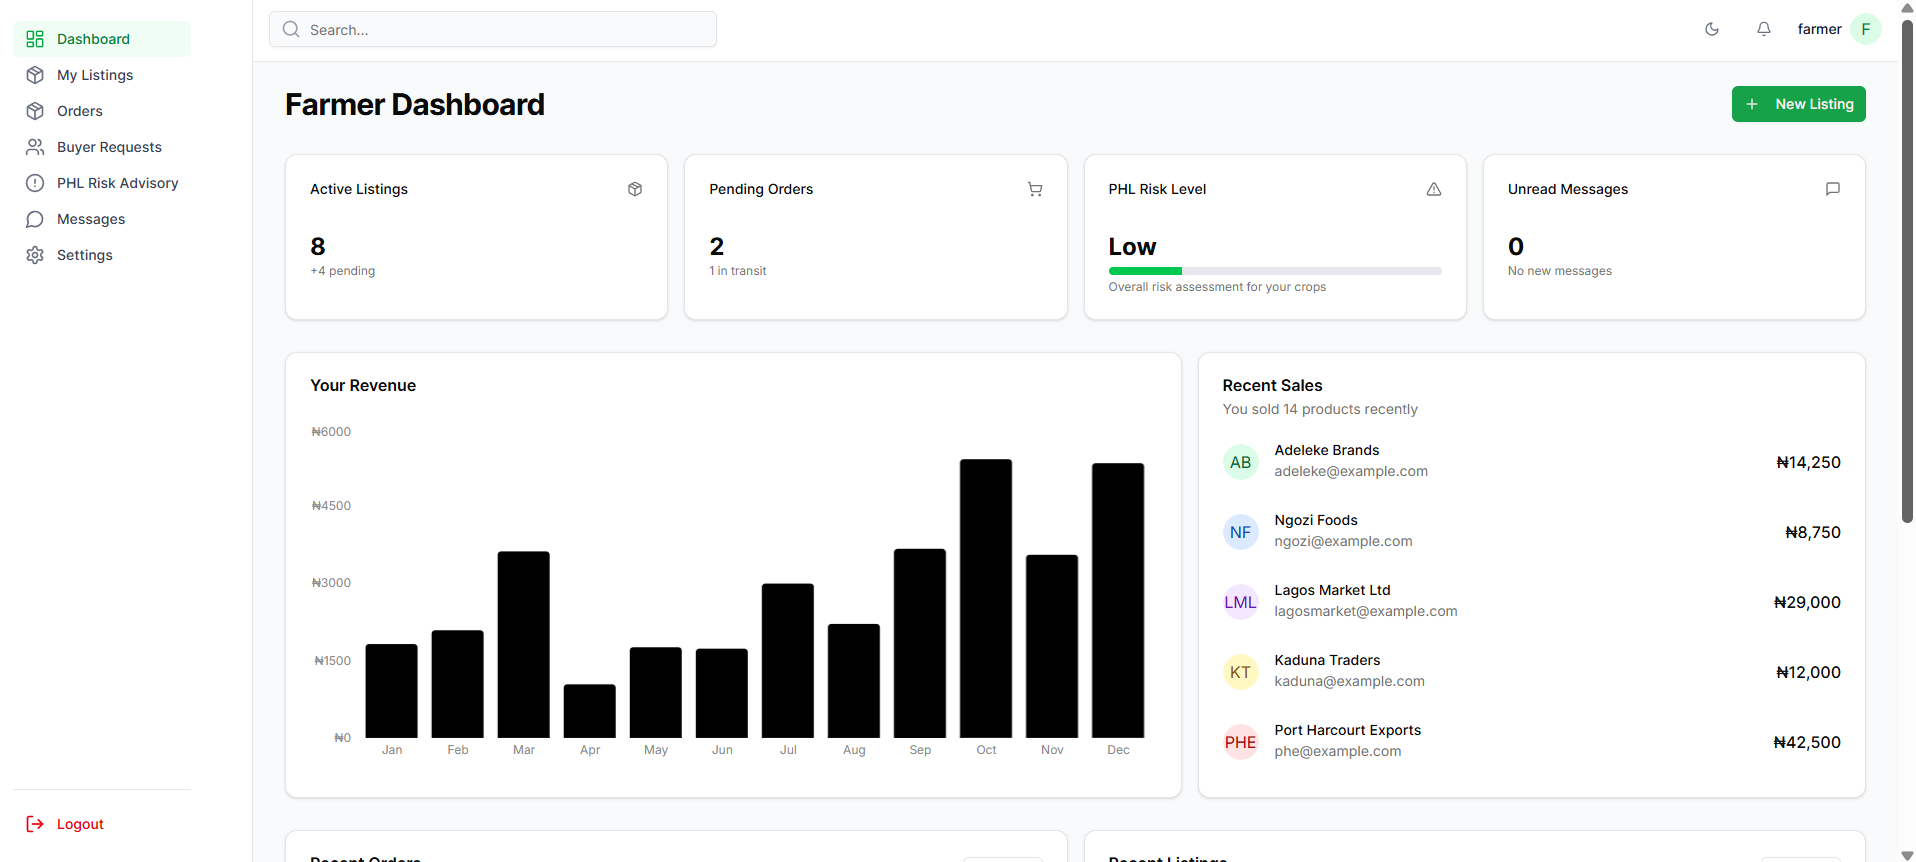
\includegraphics[scale=0.3]{Figures/okra_mockup_farmer_db.png}
    \caption{Screenshot of the farmer's dashboard}
    \label{fig:figure-06}
\end{figure}


\begin{figure}[H]
    \centering
    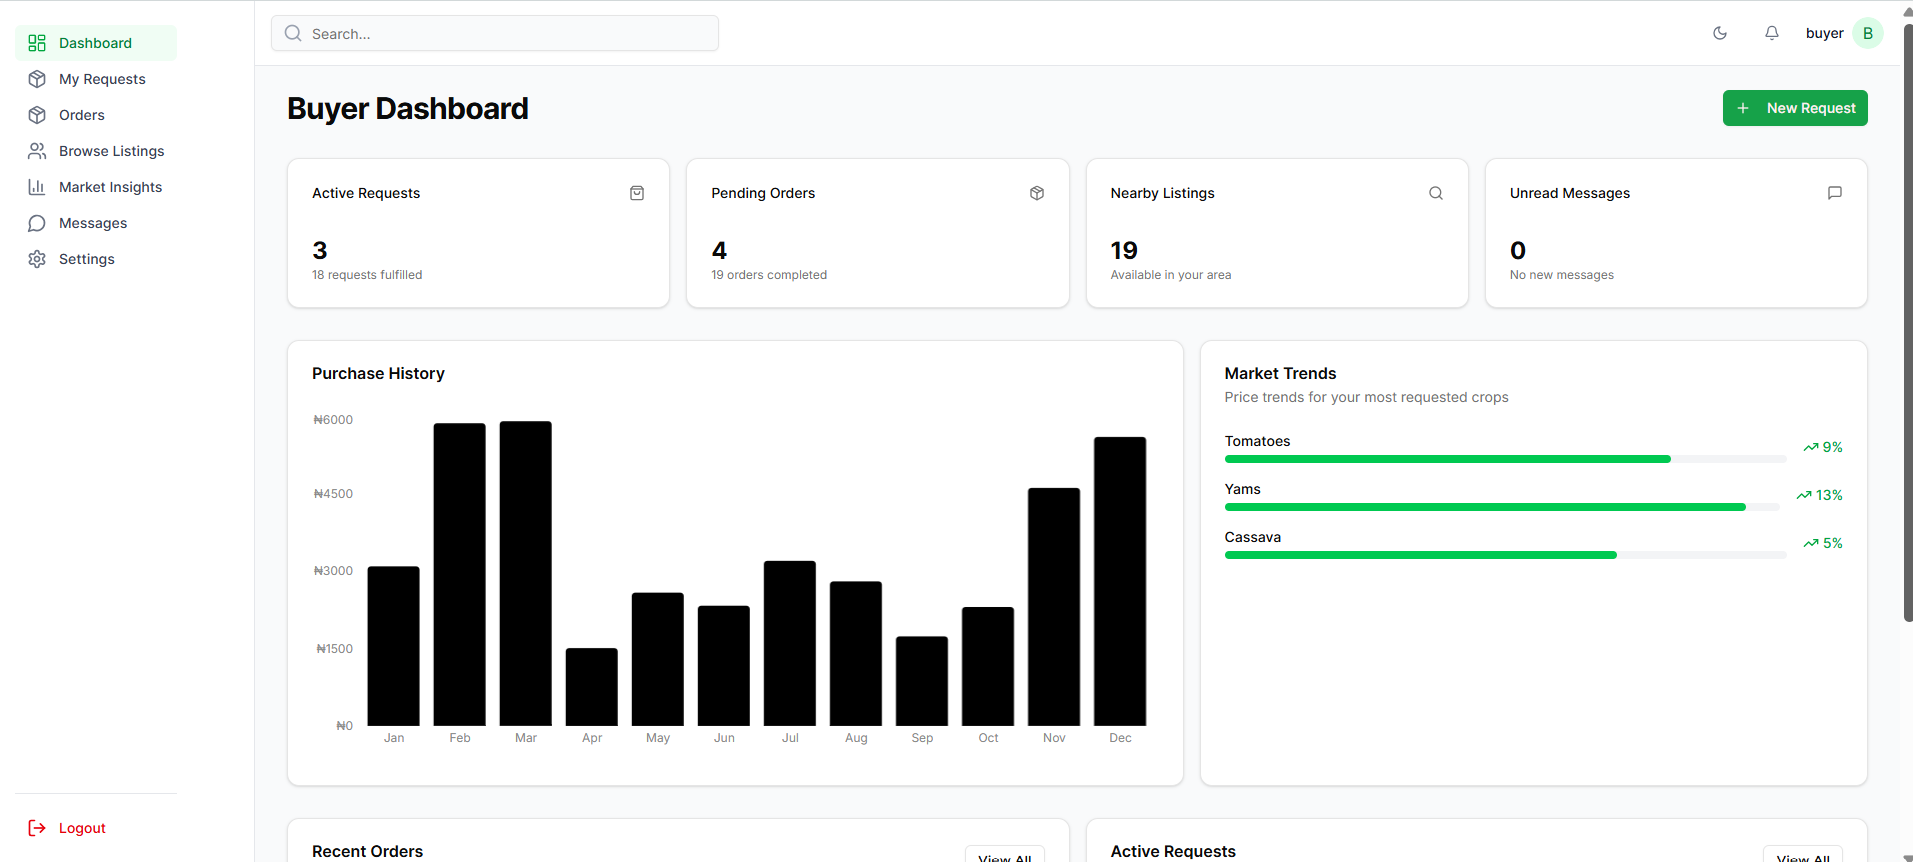
\includegraphics[scale=0.3]{Figures/okra_mockup_buyer_db.png}
    \caption{Screenshot of the buyers's dashboard}
    \label{fig:figure-07}
\end{figure}

\begin{figure}[H]
    \centering
    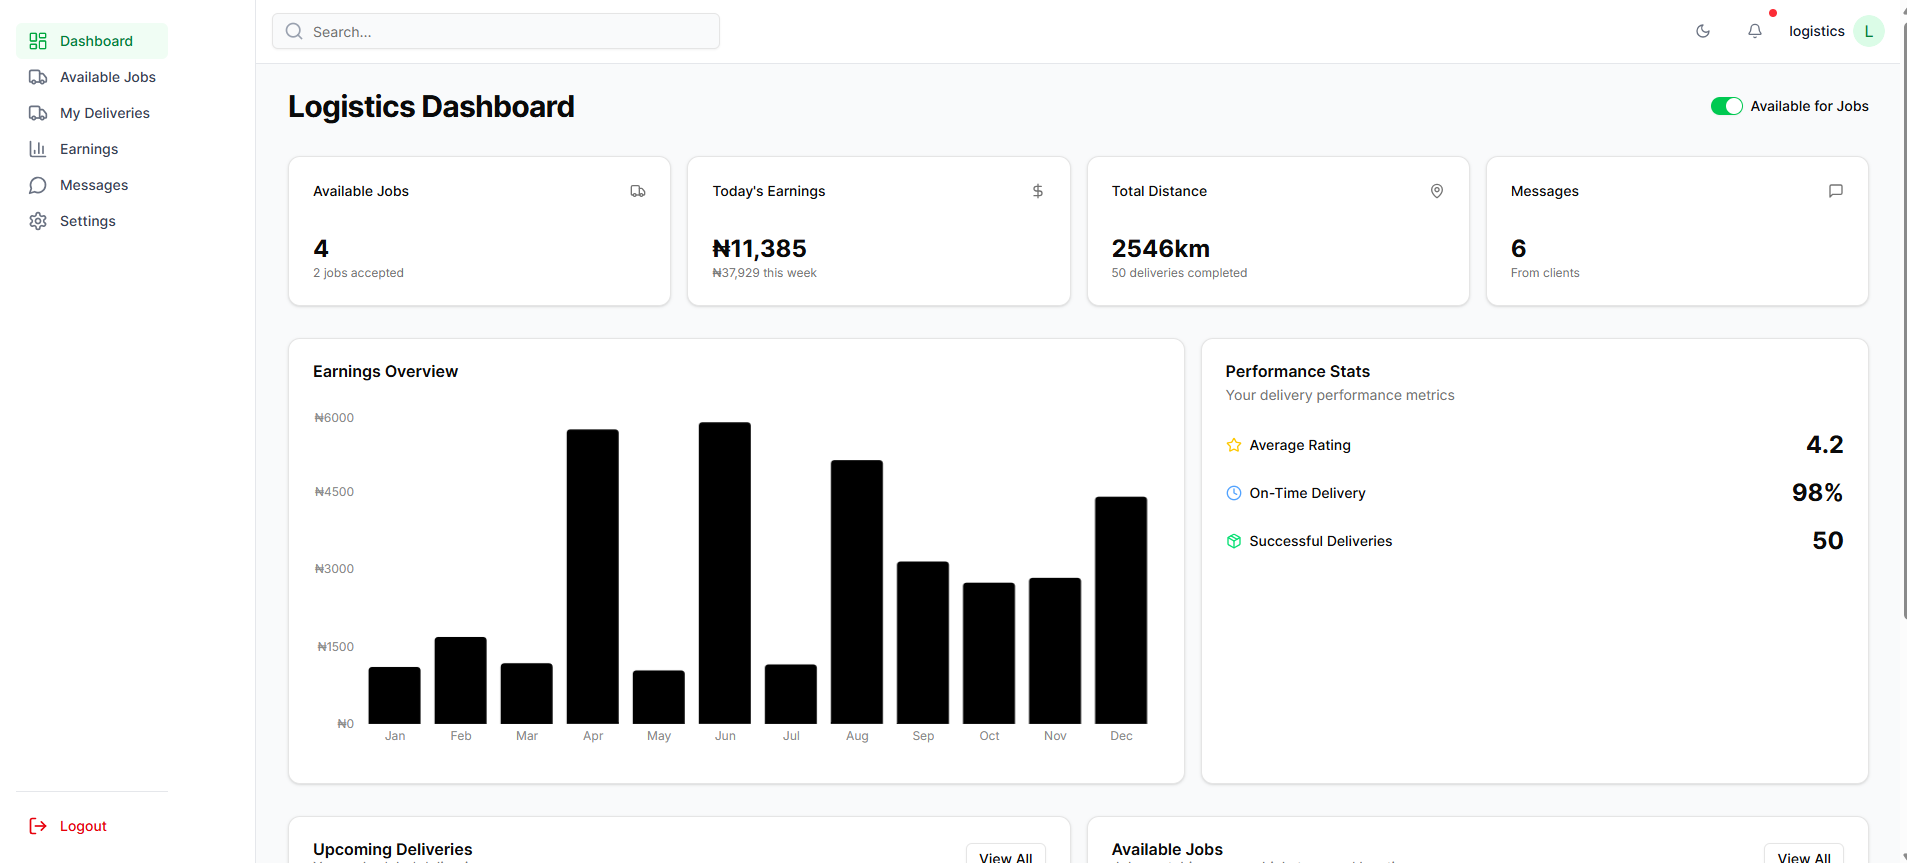
\includegraphics[scale=0.3]{Figures/okra_mockup_logistics_db.png}
    \caption{Screenshot of the buyers's dashboard}
    \label{fig:figure-08}
\end{figure}


\section{Data Strategy}

\subsection{Image Data Collection}
We will collect large numbers of labeled images of harvested produce. This will be done in phases: initially, a pilot program in a few regions (e.g. Kano for tomatoes, Adamawa for maize) will train extension agents and youth volunteers to photograph produce at harvest and at sale. Each image will be tagged with metadata (crop type, variety, region, time, moisture, storage conditions, etc.). Over time, farmers using the app will also upload photos for every batch they list, creating a growing dataset.

\subsection{Data Labeling and Training}
Using expert agronomists and community training, images will be labeled for freshness (e.g. “Fresh”, “Moderately aged”, “Spoiled”) and total count/weight. This labelled dataset feeds the computer vision model. We will employ transfer learning on convolutional neural networks so the AI can accurately assess new images it has not seen before. The initial model will be tested for accuracy and iteratively improved as more data arrives.

\subsection{Feedback Loop (Active Learning)}
Post-deployment, the app will track outcomes of predicted vs. actual. For example, if the AI predicts 10 days of shelf life but spoilage occurs in 7 days, this discrepancy is logged. Buyers and farmers can rate or report the accuracy of freshness ratings. This feedback is used to retrain the model periodically, increasing its accuracy over time. In effect, the app learns from real-world results.

\section{Auxiliary data sources}
In addition to user-generated data, the system will integrate public and commercial datasets for context. Possible sources include:


\begin{description}
    \item[Crop statistics:]  Government or FAO data on regional production volumes and seasonality for major crops.
    
    \item[Geolocation] Maps of farm locations, major roads, market centers.
    
    \item[Weather/Climate] Historical and current weather data per region, since humidity and temperature affect spoilage.
    \item[Market Prices]  Data from local commodity exchanges or market surveys, to show price trends.
    \item[Demographic Data] Farm population and sizes, to profile areas served.This external data enriches the dashboard: for instance, linking rainfall patterns to losses in maize, or highlighting regions that produce a given crop. All data is tied to time and location, enabling spatio-temporal analysis.
\end{description}

\subsection{Privacy and Governance}
Farmers’ personal data (names, exact addresses) will be protected. Only aggregate or anonymized data used on dashboards. Data use agreements will ensure that insights (e.g. “X tonnes of tomatoes sold from Kano”) respect user privacy while guiding decisions.


\section{OkraAI}
Okra features a Fruit Ripeness Prediction tool, using computer vision (CV), a specialized branch of machine learning that enables computers to analyze and interpret visual data from images. This technology facilitates the detection and prediction of fruit and vegetable freshness.

For this object detection task, the YOLOv11 model was specifically chosen due to its:

\begin{description}
    \item[Speed:] YOLOv11 is known for its fast processing speed, making it suitable for real-time applications.
    \item[Accuracy:] It achieves high accuracy in detecting and classifying objects within images.
    \item[Flexibility:] The model can be trained on various datasets, allowing it to adapt to different types of produce.
\end{description}



%     \begin{figure}[H]
%     \centering
%     \includegraphics[scale=0.1]{Figures/diagram-export-5-15-2025-5_49_16-PM.png}
%     \caption{Screenshot of the landing page}
%     \label{fig:figure-12}
% \end{figure}

\subsection{Dataset}
A hybrid dataset was constructed by combining multiple primary and secondary datasets. This approach aimed to enhance the model's generalization capabilities and ensure a broad representation of fruit ripeness stages. The dataset includes the following classes:

\begin{itemize}
  \item Ripe
  \item Unripe
  \item Rotten
\end{itemize}


Data sources include:

\begin{enumerate}
  \item \textbf{Ripe Orange Dataset}: Primary data collected and annotated by Team Okra.
  \item \textbf{Tomato Checker Dataset}: Source: Roboflow (\url{https://universe.roboflow.com/money-detection-xez0r/tomato-checker/dataset/}).
  \item \textbf{Banana Ripeness Dataset}: Source: Roboflow (\url{https://universe.roboflow.com/arm-oeppz/banana-8qkur/dataset/2}).
  \item \textbf{Rot Detection}: Source: Roboflow (\url{https://universe.roboflow.com/srmist-doq3j/rot_detection/dataset/13}).
  \item \textbf{Orange Dataset 2}: Source: Roboflow (\url{https://universe.roboflow.com/mert6107/orange_detection-5f84p/dataset/}).
\end{enumerate}


This dataset includes prevalent perishable fruits and vegetables including bananas, oranges, eggplants, garden egg, spinach, grapes, tomatoes, and cucumbers.

\section{Data Split}
The combined dataset was divided into training and validation sets using a 70:30 split.

\begin{table}[!htpb]
    \caption{Class distribution before re-splitting}
    \label{tab:image-split}
    \centering
    \begin{tabular}{lccc}
        
        \toprule
        \textbf{No. of Images} & \textbf{Ripe} & \textbf{Rotten} & \textbf{Unripe} \\
        \midrule
        Train              & 3000 & 2879 & 2105 \\
        Train Split        & 2100 & 2015 & 1473 \\
        Validation Split   & 900  & 864  & 632  \\
        \bottomrule
    \end{tabular}

\end{table}


\section{Model Training}

The pretrained YOLOv11s model was fine-tuned using the custom dataset, running with Pytorch and Ultralytics within the free tier Google Colaboratory environment. The compute environment specifications were: 112GB ROM, 12.7GB RAM, and a T4 GPU with 15GB RAM. The hyperparameters were set as follows:

\begin{description}
  \item[Model:] \texttt{yolov11s} (selected for a balance between speed and accuracy)
  \item[Epochs:] 20
  \item[Image Size:] 640
  \item[Optimizer:] AdamW (learning rate = 0.001429, momentum = 0.9)
\end{description}


The training process was completed in 0.797 hours.
The model's performance on the validation set is summarized in the table below:

\begin{table}[!htpb]
    \caption{Model performance on the validation set.}
    \label{tab:model-performance}
    \centering
    \begin{tabular}{lccccc}
       
        \toprule
        \textbf{Class} & \textbf{Images} & \textbf{Instances} & \textbf{Box(P)} & \textbf{Box(R)} & \textbf{mAP50-95} \\
        \midrule
        all    & 2396 & 3938 & 0.822 & 0.802 & 0.65 \\
        ripe   & 900  & 1077 & 0.896 & 0.949 & 0.895 \\
        rotten & 864  & 1810 & 0.703 & 0.530 & 0.332 \\
        unripe & 632  & 1051 & 0.868 & 0.928 & 0.721 \\
        \bottomrule
    \end{tabular}
        
    \vspace{0.5em}
    \textit{\textbf{Speed}: 0.2ms preprocess, 5.1ms inference, 0.0ms loss, 2.0ms postprocess per image.}
\end{table}


\section{Deployment}
The YOLOv11s model achieves a mean Average Precision (mAP50) of 0.847 and an mAP50-95 of 0.65, exceling at fruit discrimination with high precision (Box(P)) and recall (Box(R)) scores, and consequently, high mAP50 and mAP50-95 values. This indicates that the model is both accurate in its detections and effectively identifies most instances of these classes.
\vspace{\myvspace}

However, the model shows a comparatively lower performance in detecting rotten fruits. The precision (0.703) and recall (0.53) are notably lower than those for ripe and unripe categories, resulting in a lower mAP50 (0.62) and a significantly lower mAP50-95 (0.332). This suggests that the model may be less accurate in identifying rotten fruits and might miss a significant portion of them.
\vspace{\myvspace}

The inference speed of 5.1ms per image, after preprocessing and postprocessing, indicates that the model is efficient for real-time applications.

\section{Confusion Matrix}
The confusion matrix shows that the  YOLOv11s model effectively classifies ripe (1015), rotten (1034), and unripe (984) fruits, reasonably well. However, there were significant misclassifications of background as rotten (766), and some ripe (119) and unripe (147) fruits were confused with background. Despite these errors, misclassifications between ripeness categories were low, showing reliable differentiation between maturity stages. While performing well, the model's robustness could be improved by more background data and stronger regularization to reduce false positives.

    \begin{figure}[H]
    \centering
    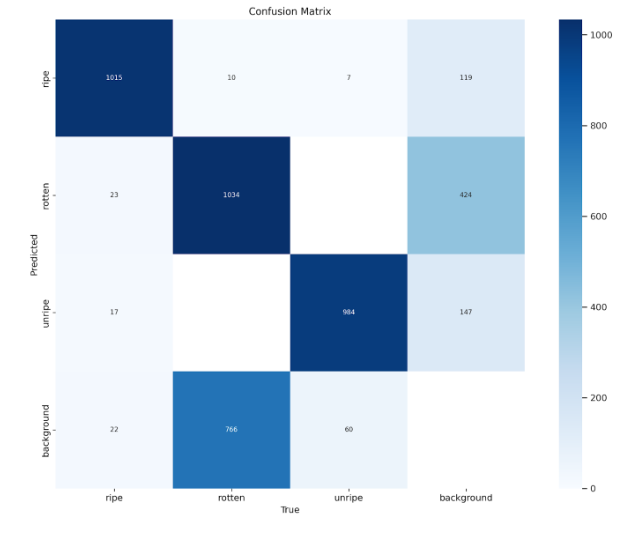
\includegraphics[scale=0.8]{Figures/confusion_matrix.png}
    \caption{Confusion matrix of the model}
    \label{fig:figure-09}
\end{figure}

\section{Training Progression}
The metric progression shows a consistent trend of improvement with increasing epochs, indicating effective learning and minimal overfitting. The proximate training and validation scores further underscore the model's generalizability to unseen images. Visual analysis reveals that at epoch 20, the terminal iteration, the model attains optimal performance, displaying the nadir of loss values and the apex of mean Average Precision (mAP), Precision, and Recall scores.

    \begin{figure}[H]
    \centering
    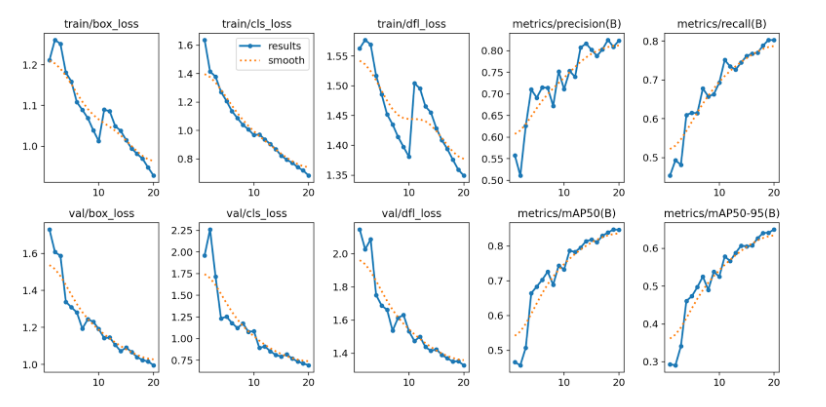
\includegraphics[scale=0.8]{Figures/training.png}
    \caption{Training progression of the model}
    \label{fig:figure-10}
\end{figure}


\section{F1-Confidence Curve}
The F1-confidence curve in \autoref{fig:figure-11} illustrates the F1-score across various confidence thresholds. A higher F1-score indicates a more effective model in differentiating between the dataset's classes. Our model achieves a peak F1-score of 0.81 (81\%) at a confidence threshold of 0.278. This suggests that for optimal deployment, the recommended confidence threshold should be approximately 0.3.

    \begin{figure}[H]
    \centering
    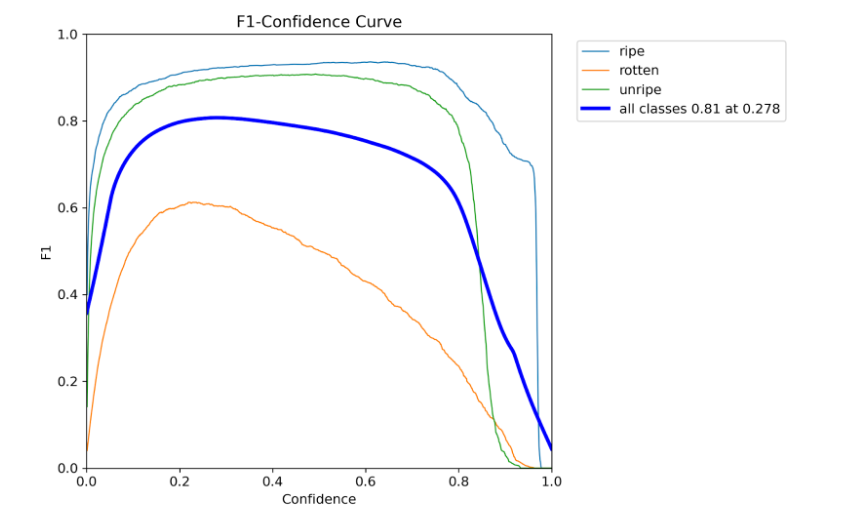
\includegraphics[scale=0.8]{Figures/fi_conf.png}
    \caption{F1-confidence curve of the model}
    \label{fig:figure-11}
\end{figure}


\section{Deployment and Demo}
For integration into the Okra app, the trained YOLOv11s model was exported to the ONNX (Open Neural Network Exchange) format \citep{onnx}. ONNX is a widely supported format for representing neural network architectures, facilitating deployment across diverse platforms such as mobile devices, web applications, microcontrollers, and servers.
\vspace{\myvspace}

To showcase the model's capabilities, a demonstration web application was developed using the Gradio tool. Images illustrating the model in operation are provided below.

% {insert gradio demo images on the group} 
%     \begin{figure}[H]
%     \centering
%     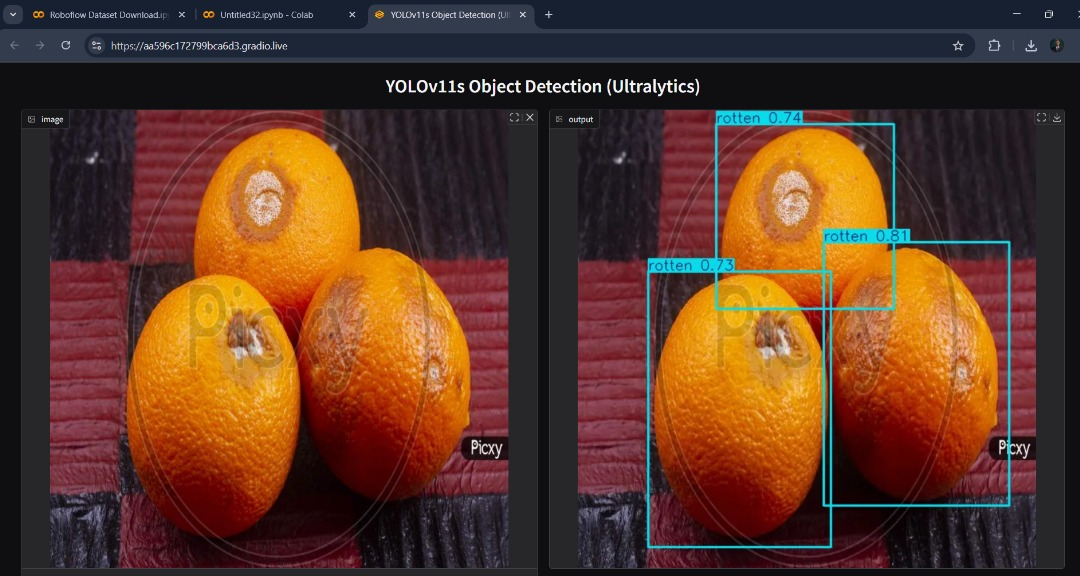
\includegraphics[scale=0.4]{Figures/gradio_demo_1.jpg}
%     \caption{Confusion matrix of the model}
%     \label{fig:figure-12}
% \end{figure}


\begin{figure}[!htpb]
    \centering
    \begin{subfigure}{0.45\textwidth}
        \centering
        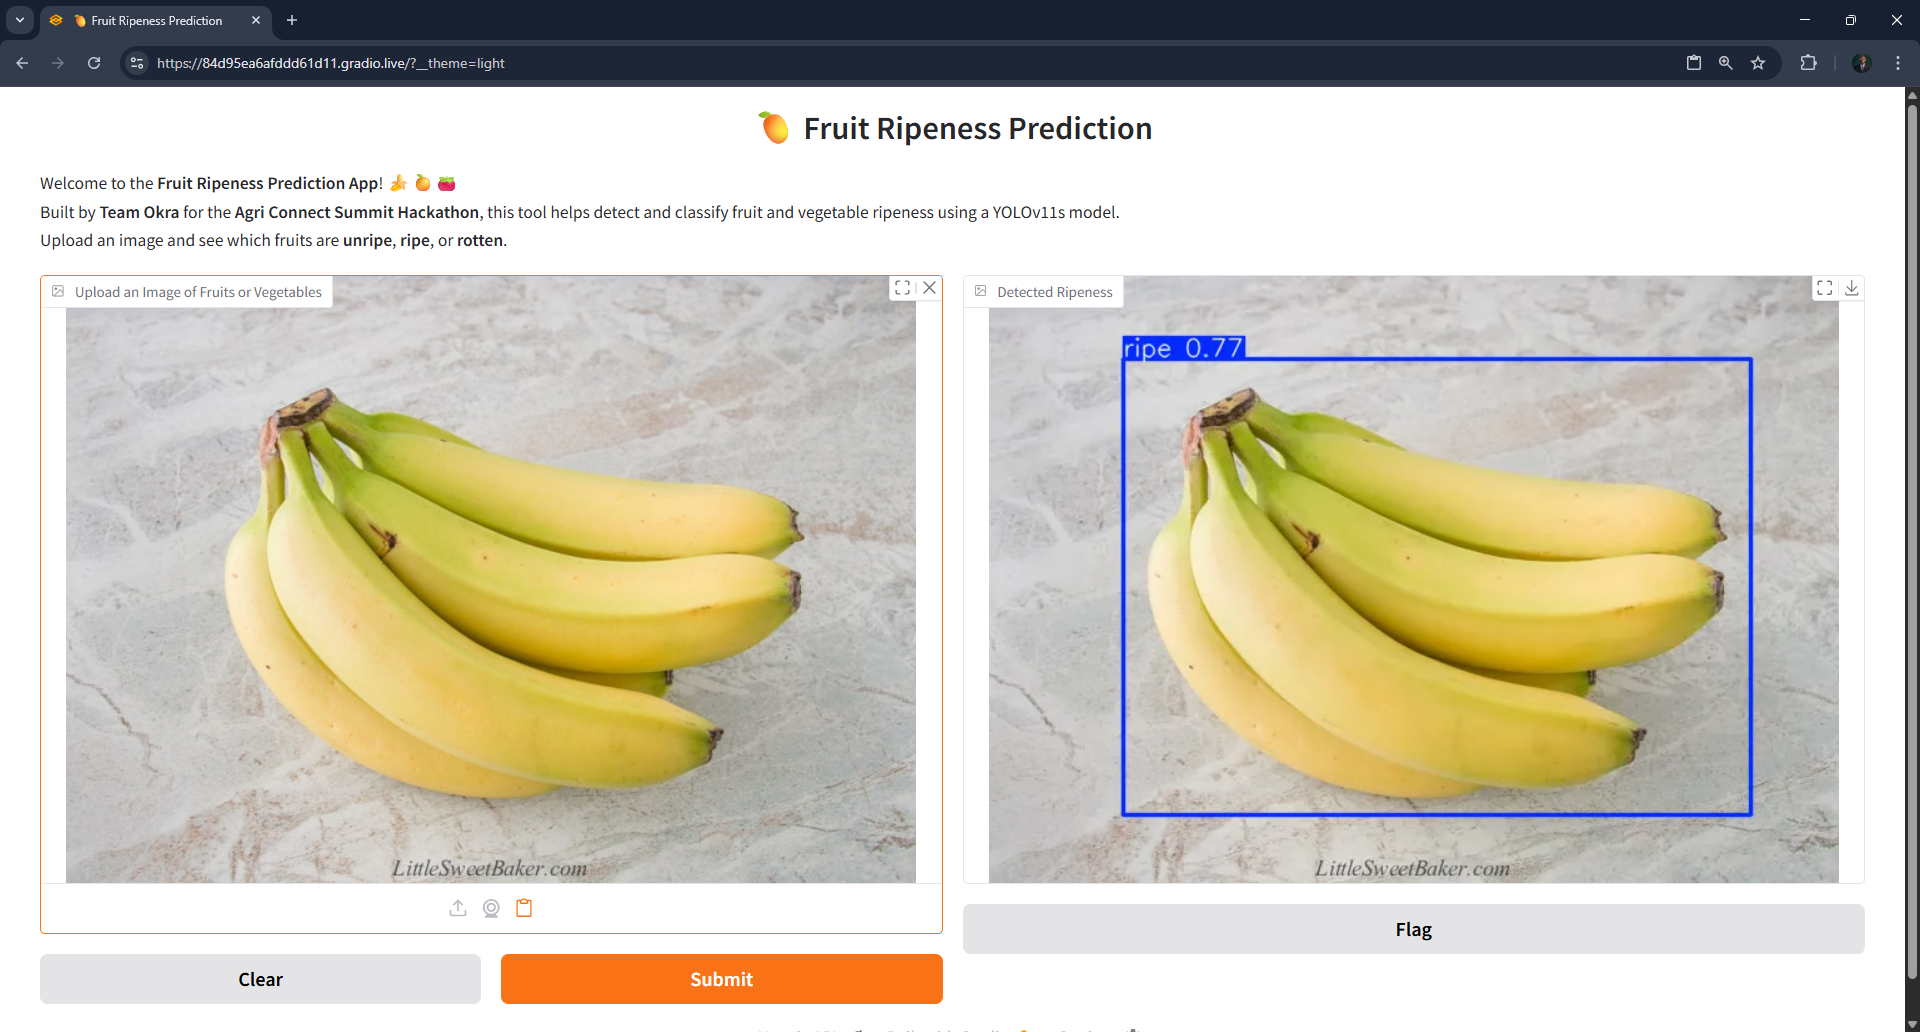
\includegraphics[width=0.9\textwidth]{Figures/gradio_demo_1.png}
        \caption{Gradio Demo 1}
        \label{fig:figure-12.1}
    \end{subfigure}
    \hspace{.5cm} % Adjust the space as needed.
    \begin{subfigure}{0.45\textwidth}
        \centering
        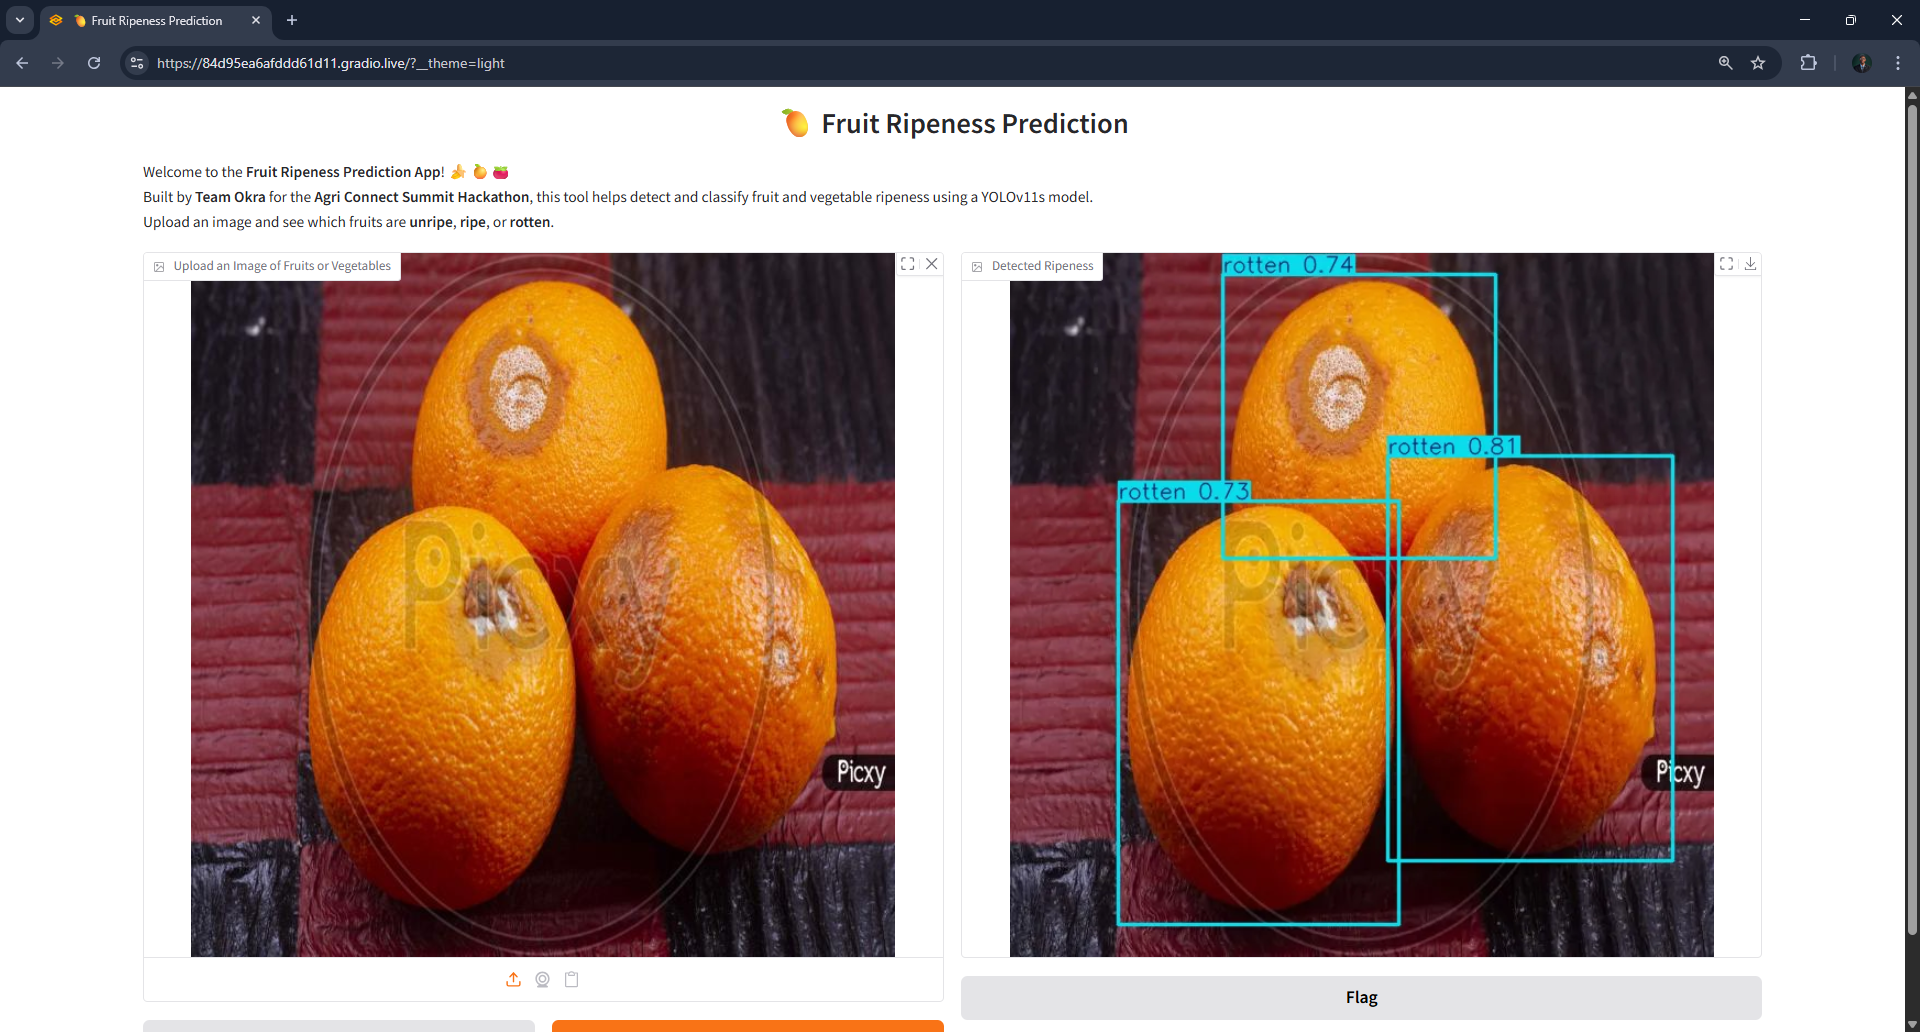
\includegraphics[width=0.9\textwidth]{Figures/gradio_demo_2.png}
        \caption{Gradio Demo 2}
        \label{fig:figure-12.2}
    \end{subfigure}
    \caption{Gradio Demo of the model}
    \label{fig:figure-12}
\end{figure}



}